\documentclass{standalone}
\usepackage{tikz}
\usetikzlibrary{patterns, positioning}


\begin{document}
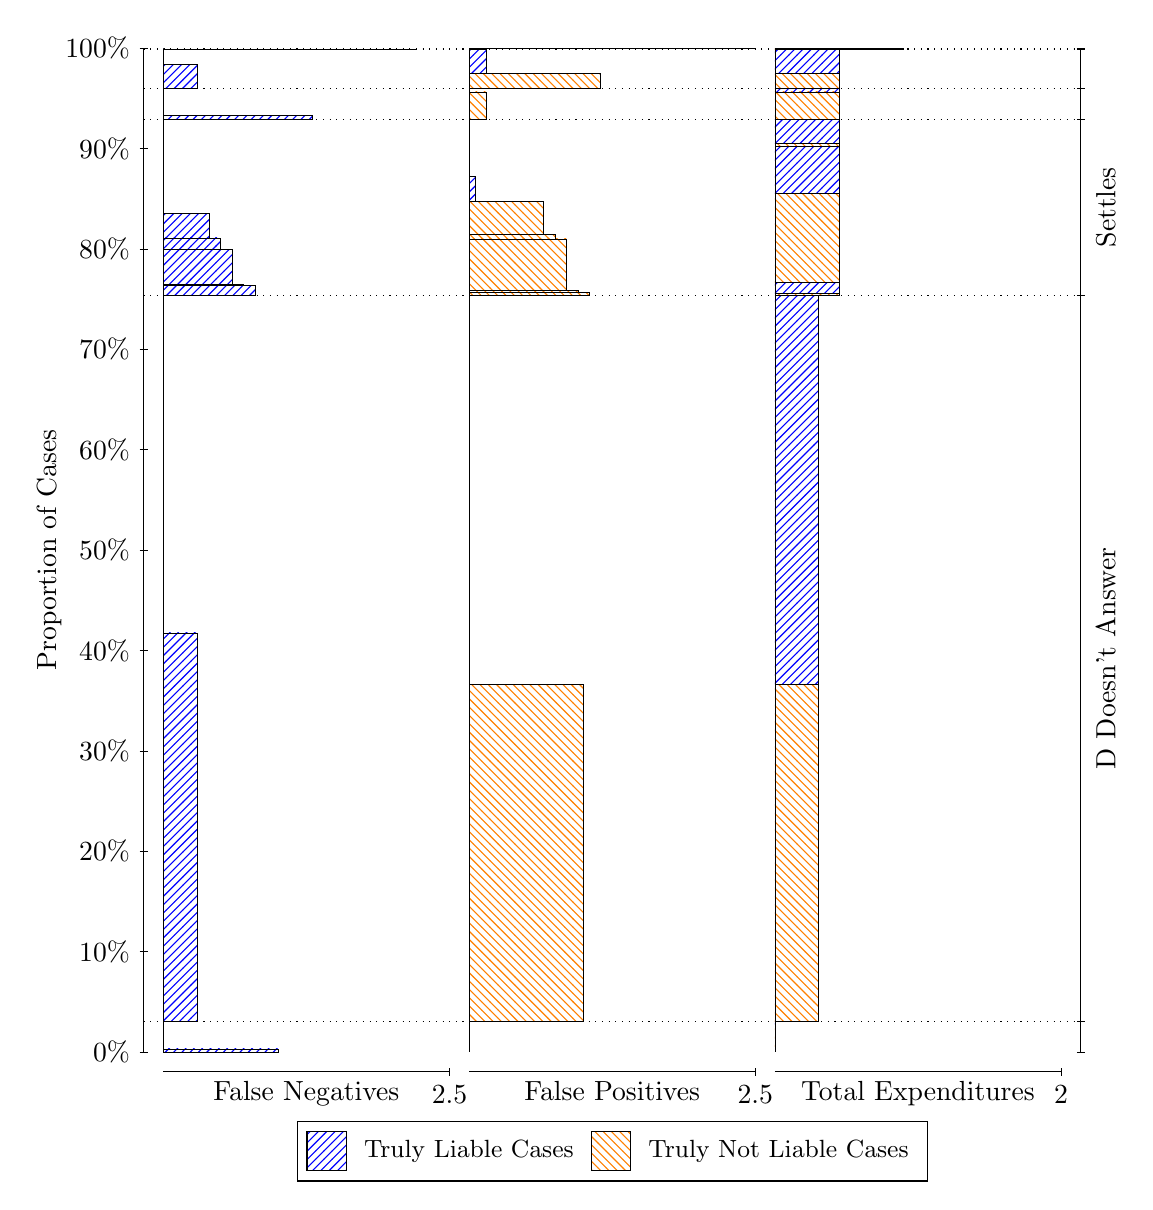
\begin{tikzpicture}
\draw[black, very thin] (1.5,1.75) -- (1.5,14.5);
\node[rotate=90, text=black, anchor=center] at (0.3, 8.125) {Proportion of Cases};
\draw[black, very thin] (1.45,1.75) -- (1.55,1.75);
\node[text=black, anchor=east] at (1.45, 1.75) {0\%};
\draw[black, very thin] (1.45,3.025) -- (1.55,3.025);
\node[text=black, anchor=east] at (1.45, 3.025) {10\%};
\draw[black, very thin] (1.45,4.3) -- (1.55,4.3);
\node[text=black, anchor=east] at (1.45, 4.3) {20\%};
\draw[black, very thin] (1.45,5.575) -- (1.55,5.575);
\node[text=black, anchor=east] at (1.45, 5.575) {30\%};
\draw[black, very thin] (1.45,6.85) -- (1.55,6.85);
\node[text=black, anchor=east] at (1.45, 6.85) {40\%};
\draw[black, very thin] (1.45,8.125) -- (1.55,8.125);
\node[text=black, anchor=east] at (1.45, 8.125) {50\%};
\draw[black, very thin] (1.45,9.4) -- (1.55,9.4);
\node[text=black, anchor=east] at (1.45, 9.4) {60\%};
\draw[black, very thin] (1.45,10.675) -- (1.55,10.675);
\node[text=black, anchor=east] at (1.45, 10.675) {70\%};
\draw[black, very thin] (1.45,11.95) -- (1.55,11.95);
\node[text=black, anchor=east] at (1.45, 11.95) {80\%};
\draw[black, very thin] (1.45,13.225) -- (1.55,13.225);
\node[text=black, anchor=east] at (1.45, 13.225) {90\%};
\draw[black, very thin] (1.45,14.5) -- (1.55,14.5);
\node[text=black, anchor=east] at (1.45, 14.5) {100\%};

\draw[black, very thin] (13.4,1.75) -- (13.4,14.5);
\draw[black, very thin] (13.35,1.75) -- (13.45,1.75);
\node[anchor=west] at (13.35, 1.75) {};
\draw[black, very thin] (13.35,2.1348) -- (13.45,2.1348);
\node[anchor=west] at (13.35, 2.1348) {};
\draw[black, very thin] (13.35,11.358) -- (13.45,11.358);
\node[anchor=west] at (13.35, 11.358) {};
\draw[black, very thin] (13.35,13.597) -- (13.45,13.597);
\node[anchor=west] at (13.35, 13.597) {};
\draw[black, very thin] (13.35,13.986) -- (13.45,13.986);
\node[anchor=west] at (13.35, 13.986) {};
\draw[black, very thin] (13.35,14.484) -- (13.45,14.484);
\node[anchor=west] at (13.35, 14.484) {};
\draw[black, very thin] (13.35,14.495) -- (13.45,14.495);
\node[anchor=west] at (13.35, 14.495) {};
\draw[black, very thin] (13.35,14.5) -- (13.45,14.5);
\node[anchor=west] at (13.35, 14.5) {};

\draw[black, very thin, pattern color=blue, pattern=north east lines] (1.75,1.75) rectangle (3.2033,1.7905);
\draw[black, very thin, pattern color=orange, pattern=north west lines] (1.75,1.7905) rectangle (1.75,2.1348);
\draw[black, very thin, pattern color=blue, pattern=north east lines] (1.75,2.1348) rectangle (2.186,7.0717);
\draw[black, very thin, pattern color=orange, pattern=north west lines] (1.75,7.0717) rectangle (1.75,11.358);
\draw[black, very thin, pattern color=blue, pattern=north east lines] (1.75,11.358) rectangle (2.9127,11.489);
\draw[black, very thin, pattern color=blue, pattern=north east lines] (1.75,11.489) rectangle (2.7673,11.494);
\draw[black, very thin, pattern color=blue, pattern=north east lines] (1.75,11.494) rectangle (2.622,11.947);
\draw[black, very thin, pattern color=blue, pattern=north east lines] (1.75,11.947) rectangle (2.4767,12.088);
\draw[black, very thin, pattern color=blue, pattern=north east lines] (1.75,12.088) rectangle (2.3313,12.4);
\draw[black, very thin, pattern color=orange, pattern=north west lines] (1.75,12.4) rectangle (1.75,13.597);
\draw[black, very thin, pattern color=blue, pattern=north east lines] (1.75,13.597) rectangle (3.6393,13.641);
\draw[black, very thin, pattern color=orange, pattern=north west lines] (1.75,13.641) rectangle (1.75,13.986);
\draw[black, very thin, pattern color=blue, pattern=north east lines] (1.75,13.986) rectangle (2.186,14.292);
\draw[black, very thin, pattern color=orange, pattern=north west lines] (1.75,14.292) rectangle (1.75,14.484);
\draw[black, very thin, pattern color=blue, pattern=north east lines] (1.75,14.484) rectangle (4.9473,14.487);
\draw[black, very thin, pattern color=orange, pattern=north west lines] (1.75,14.487) rectangle (1.75,14.495);
\draw[black, very thin, pattern color=orange, pattern=north west lines] (1.75,14.495) rectangle (1.75,14.497);
\draw[black, very thin, pattern color=blue, pattern=north east lines] (1.75,14.497) rectangle (1.75,14.5);
\draw[black, very thin, pattern color=orange, pattern=north west lines] (5.6333,1.75) rectangle (5.6333,2.0943);
\draw[black, very thin, pattern color=blue, pattern=north east lines] (5.6333,2.0943) rectangle (5.6333,2.1348);
\draw[black, very thin, pattern color=orange, pattern=north west lines] (5.6333,2.1348) rectangle (7.0867,6.4212);
\draw[black, very thin, pattern color=blue, pattern=north east lines] (5.6333,6.4212) rectangle (5.6333,11.358);
\draw[black, very thin, pattern color=orange, pattern=north west lines] (5.6333,11.358) rectangle (7.1593,11.396);
\draw[black, very thin, pattern color=orange, pattern=north west lines] (5.6333,11.396) rectangle (7.014,11.418);
\draw[black, very thin, pattern color=orange, pattern=north west lines] (5.6333,11.418) rectangle (6.8687,12.075);
\draw[black, very thin, pattern color=orange, pattern=north west lines] (5.6333,12.075) rectangle (6.7233,12.134);
\draw[black, very thin, pattern color=orange, pattern=north west lines] (5.6333,12.134) rectangle (6.578,12.555);
\draw[black, very thin, pattern color=blue, pattern=north east lines] (5.6333,12.555) rectangle (5.706,12.867);
\draw[black, very thin, pattern color=blue, pattern=north east lines] (5.6333,12.867) rectangle (5.6333,13.597);
\draw[black, very thin, pattern color=orange, pattern=north west lines] (5.6333,13.597) rectangle (5.8513,13.942);
\draw[black, very thin, pattern color=blue, pattern=north east lines] (5.6333,13.942) rectangle (5.6333,13.986);
\draw[black, very thin, pattern color=orange, pattern=north west lines] (5.6333,13.986) rectangle (7.3047,14.178);
\draw[black, very thin, pattern color=blue, pattern=north east lines] (5.6333,14.178) rectangle (5.8513,14.484);
\draw[black, very thin, pattern color=orange, pattern=north west lines] (5.6333,14.484) rectangle (5.6333,14.492);
\draw[black, very thin, pattern color=blue, pattern=north east lines] (5.6333,14.492) rectangle (5.6333,14.495);
\draw[black, very thin, pattern color=orange, pattern=north west lines] (5.6333,14.495) rectangle (9.2667,14.497);
\draw[black, very thin, pattern color=blue, pattern=north east lines] (5.6333,14.497) rectangle (7.8133,14.5);
\draw[black, very thin, pattern color=orange, pattern=north west lines] (9.5167,1.75) rectangle (9.5167,2.0943);
\draw[black, very thin, pattern color=blue, pattern=north east lines] (9.5167,2.0943) rectangle (9.5167,2.1348);
\draw[black, very thin, pattern color=orange, pattern=north west lines] (9.5167,2.1348) rectangle (10.062,6.4212);
\draw[black, very thin, pattern color=blue, pattern=north east lines] (9.5167,6.4212) rectangle (10.062,11.358);
\draw[black, very thin, pattern color=orange, pattern=north west lines] (9.5167,11.358) rectangle (10.334,11.38);
\draw[black, very thin, pattern color=blue, pattern=north east lines] (9.5167,11.38) rectangle (10.334,11.521);
\draw[black, very thin, pattern color=orange, pattern=north west lines] (9.5167,11.521) rectangle (10.334,12.658);
\draw[black, very thin, pattern color=blue, pattern=north east lines] (9.5167,12.658) rectangle (10.334,13.247);
\draw[black, very thin, pattern color=orange, pattern=north west lines] (9.5167,13.247) rectangle (10.334,13.285);
\draw[black, very thin, pattern color=blue, pattern=north east lines] (9.5167,13.285) rectangle (10.334,13.597);
\draw[black, very thin, pattern color=orange, pattern=north west lines] (9.5167,13.597) rectangle (10.334,13.942);
\draw[black, very thin, pattern color=blue, pattern=north east lines] (9.5167,13.942) rectangle (10.334,13.986);
\draw[black, very thin, pattern color=orange, pattern=north west lines] (9.5167,13.986) rectangle (10.334,14.178);
\draw[black, very thin, pattern color=blue, pattern=north east lines] (9.5167,14.178) rectangle (10.334,14.484);
\draw[black, very thin, pattern color=orange, pattern=north west lines] (9.5167,14.484) rectangle (11.152,14.492);
\draw[black, very thin, pattern color=blue, pattern=north east lines] (9.5167,14.492) rectangle (11.152,14.495);
\draw[black, very thin, pattern color=orange, pattern=north west lines] (9.5167,14.495) rectangle (11.152,14.497);
\draw[black, very thin, pattern color=blue, pattern=north east lines] (9.5167,14.497) rectangle (11.152,14.5);
\draw[black, dotted] (1.5,2.1348) -- (13.4,2.1348);
\draw[black, dotted] (1.5,11.358) -- (13.4,11.358);
\draw[black, dotted] (1.5,13.597) -- (13.4,13.597);
\draw[black, dotted] (1.5,13.986) -- (13.4,13.986);
\draw[black, dotted] (1.5,14.484) -- (13.4,14.484);
\draw[black, dotted] (1.5,14.495) -- (13.4,14.495);
\draw[black, very thin] (1.75,1.5) -- (5.3833,1.5);
\node[text=black, anchor=north] at (3.5667, 1.5) {False Negatives};
\draw[black, very thin] (5.3833,1.45) -- (5.3833,1.55);
\node[text=black, anchor=north] at (5.3833, 1.45) {2.5};

\draw[black, very thin] (5.6333,1.5) -- (9.2667,1.5);
\node[text=black, anchor=north] at (7.45, 1.5) {False Positives};
\draw[black, very thin] (9.2667,1.45) -- (9.2667,1.55);
\node[text=black, anchor=north] at (9.2667, 1.45) {2.5};

\draw[black, very thin] (9.5167,1.5) -- (13.15,1.5);
\node[text=black, anchor=north] at (11.333, 1.5) {Total Expenditures};
\draw[black, very thin] (13.15,1.45) -- (13.15,1.55);
\node[text=black, anchor=north] at (13.15, 1.45) {2};


\node[text=black, centered, rotate=90] at (13.72, 6.7465) {D Doesn't Answer};
\node[text=black, centered, rotate=90] at (13.72, 12.478) {Settles};





\draw (7.449999999999999,1.5) node[draw=none] (baseCoordinate) {};
\begin{scope}[align=center]
        \matrix[scale=0.5, draw=black, below=0.5cm of baseCoordinate, nodes={draw}, column sep=0.1cm]{
            \node[rectangle, draw, minimum width=0.5cm, minimum height=0.5cm, pattern color=blue, pattern=north east lines] {}; &
            \node[draw=none, font=\small, text=black] (B) {Truly Liable Cases}; &
            \node[rectangle, draw, minimum width=0.5cm, minimum height=0.5cm, pattern color=orange, pattern=north west lines] {}; &
            \node[draw=none, font=\small, text=black] (B) {Truly Not Liable Cases}; \\
            };
\end{scope}

\end{tikzpicture}
\end{document}